\documentclass[border=10pt]{standalone}

% --- packages (mirror these in figure.meta.json "requires") ---
\usepackage{tikz}
\usetikzlibrary{positioning, arrows.meta, shapes.symbols, fit, backgrounds}

% --- palette (canonical source: reference/color-palettes/color-palettes.md; light variant) ---
\definecolor{otblue}{HTML}{0072B2}
\definecolor{otorange}{HTML}{E69F00}
\definecolor{otteal}{HTML}{009E73}
\definecolor{otpurple}{HTML}{CC79A7}
\definecolor{otgray}{HTML}{5A5A5A}

% ===== reusable icon sub-pictures (adapted from icons/) ==================
\newcommand{\cloudpic}{%
  
\begin{tikzpicture}
    \node[cloud, cloud puffs=11, cloud puff arc=110, aspect=2.2,
      draw=otblue!75!black, fill=otblue!15, line width=0.7pt,
      minimum width=2cm, minimum height=1.2cm]{};
  \end{tikzpicture}}
\newcommand{\serverpic}{%
  
\begin{tikzpicture}[line width=0.55pt]
    \foreach \i in {0,1,2}{
      \filldraw[draw=otblue!75!black, fill=otblue!12, rounded corners=1pt]
        (0,\i*0.34) rectangle (1.0,\i*0.34+0.26);
      \filldraw[otteal] (0.13,\i*0.34+0.13) circle[radius=0.04];
    }
  \end{tikzpicture}}
\newcommand{\gpupic}{%
  
\begin{tikzpicture}[line width=0.5pt]
    \filldraw[draw=otteal!70!black, fill=otteal!12, rounded corners=1pt] (0,0) rectangle (1.0,0.62);
    \begin{scope}[shift={(0.31,0.31)}]
      \filldraw[draw=otteal!75!black, fill=otteal!22] (0,0) circle[radius=0.17];
      \foreach \a in {0,90,180,270}{\draw[otteal!70!black, line width=0.4pt] (0,0)--(\a:0.15);}
    \end{scope}
    \node[font=\sffamily\tiny\bfseries, text=otteal!80!black] at (0.74,0.31){GPU};
  \end{tikzpicture}}
\newcommand{\dbpic}{%
  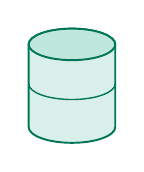
\begin{tikzpicture}[line width=0.7pt]
    \def\rx{0.55}\def\ry{0.20}\def\bh{1.05}
    \filldraw[draw=otteal!75!black, fill=otteal!15]
      (-\rx,0)--(-\rx,-\bh) arc[start angle=180,end angle=360,x radius=\rx,y radius=\ry]
      --(\rx,0) arc[start angle=0,end angle=180,x radius=\rx,y radius=\ry]--cycle;
    \filldraw[draw=otteal!75!black, fill=otteal!25] (0,0) ellipse[x radius=\rx,y radius=\ry];
    \draw[draw=otteal!75!black, line width=0.5pt]
      (-\rx,-0.5) arc[start angle=180,end angle=360,x radius=\rx,y radius=\ry];
  \end{tikzpicture}}
% ========================================================================

\begin{document}
% ==== parameters (edit these) ============================================
\def\colsep{3.0}    % horizontal gap between stages: client -> cloud -> lb -> nodes -> store (cm)
\def\rowsep{1.5}    % vertical offset of the stacked inference nodes (cm)
% labels
\def\clientlabel{Client}
\def\internetlabel{Internet}
\def\lblabel{Load\\balancer}
\def\nodeonelabel{Inference node 1}
\def\nodetwolabel{Inference node 2}
\def\storelabel{Feature store}
\def\featurelabel{features}
\def\clusterlabel{Inference cluster}
\def\titlelabel{Model inference serving}
% =========================================================================

\begin{tikzpicture}[
    >={Stealth[length=2.4mm]},
    icon/.style={inner sep=1pt},
    compbox/.style={draw=otgray!55, rounded corners=3pt, fill=otgray!8,
      align=center, font=\sffamily\small, minimum height=0.9cm, inner sep=5pt},
    nodebox/.style={draw=otgray!45, rounded corners=4pt, fill=otgray!4, inner sep=5pt},
    slbl/.style={font=\sffamily\footnotesize, text=otgray},
    req/.style={draw=otgray!75, line width=1pt, ->},
    read/.style={draw=otteal!70!black, line width=1pt, ->, dashed},
  ]

  \node[compbox] (client) at (0,0) {\clientlabel};
  \node[icon] (cloud) at (\colsep,0) {\cloudpic};
  \node[slbl, below=0pt of cloud] {\internetlabel};
  \node[compbox] (lb) at (2*\colsep,0) {\lblabel};

  % GPU-backed inference nodes (server + gpu composed in one box)
  \node[nodebox] (node1) at (3*\colsep,\rowsep)  {\serverpic\hspace{4pt}\gpupic};
  \node[nodebox] (node2) at (3*\colsep,-\rowsep) {\serverpic\hspace{4pt}\gpupic};
  \node[slbl, below=1pt of node1] (n1lab) {\nodeonelabel};
  \node[slbl, below=1pt of node2] (n2lab) {\nodetwolabel};

  \node[icon] (db) at (4.3*\colsep,0) {\dbpic};
  \node[slbl, below=2pt of db] {\storelabel};

  % request path
  \draw[req] (client.east) -- (cloud.west);
  \draw[req] (cloud.east) -- (lb.west);
  \draw[req] (lb.east) -- (node1.west);
  \draw[req] (lb.east) -- (node2.west);
  % feature reads
  \draw[read] (node1.east) -- (db.west);
  \draw[read] (node2.east) -- (db.west);
  \node[slbl, text=otteal!70!black] at (3.85*\colsep,0.55) {\featurelabel};

  % inference cluster boundary (fits the nodes and their labels)
  \begin{scope}[on background layer]
    \node[draw=otgray!50, dashed, rounded corners=6pt, fill=otgray!4, inner sep=10pt,
          fit=(node1)(node2)(n1lab)(n2lab)] (cluster) {};
    \node[slbl, anchor=south west] at ([xshift=2pt, yshift=2pt]cluster.north west) {\clusterlabel};
  \end{scope}

  % title
  \node[font=\sffamily\bfseries] at (2.17*\colsep,{\rowsep+1.7}) {\titlelabel};

\end{tikzpicture}
\end{document}
